\documentclass[./standalone.tex]{subfiles}
%\documentclass[../../../CR/pac.tex]{subfiles}

\begin{document}

% --------------------- %
%          PART         %
% --------------------- %
\part{Manuel du joueur}

% Section:
\section{Qu'est-ce que Silent In Space?}
Silent In Space (abrégé : “SIS”) est un jeu Point \& Click dans la veine des Monkey Island. Dans ce jeu, vous vous réveillez dans un vaisseau alien et avez pour but de vous en échapper. Faites vous des alliés ou des ennemis sur votre chemin et découvrez pourquoi vous êtes ici ! 

% Section:
\section{Lancer le jeu}


\newpage

% Subsection:
\section{Les contrôles du jeu}

\begin{tabular}{| m{40em} |}
\hline
	\begin{center}
	   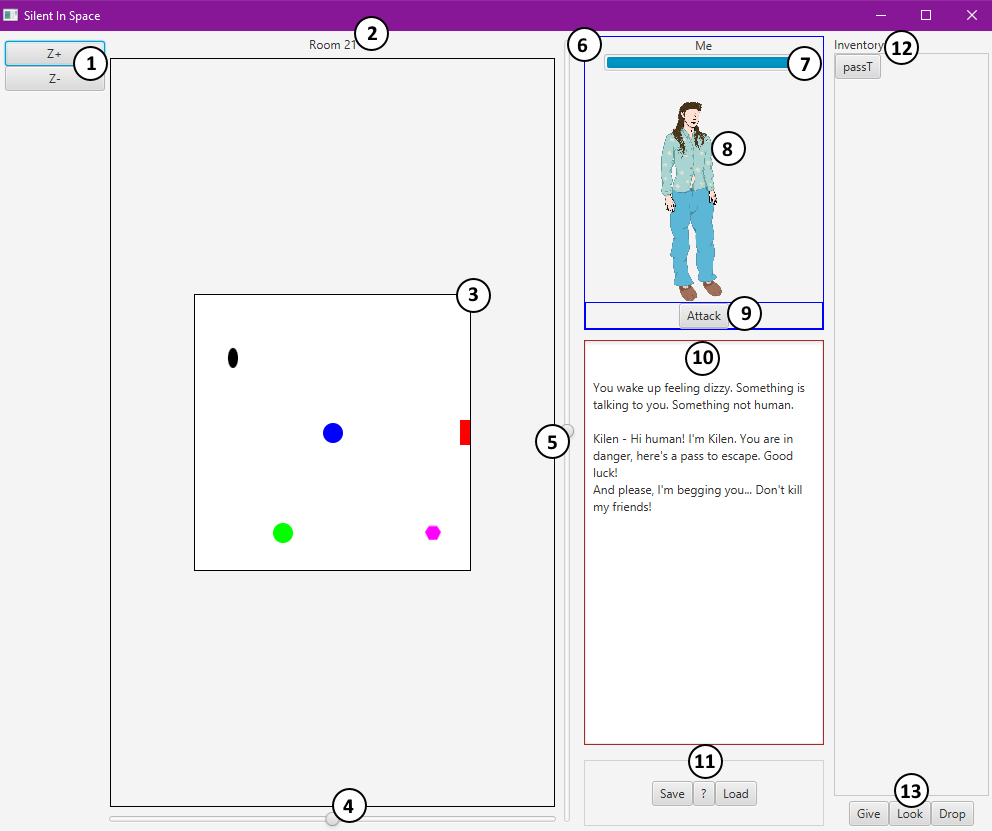
\includegraphics[scale=0.4]{images/UI.png}
	\end{center}\\
\hline
	\begin{enumerate}
		\item Fonctions de Zoom sur la carte
		\item Numéro de la pièce actuelle
		\item Panneau de la Carte de Jeu. C’est ici qu’évoluera la vue des pièces et leurs contenus
		
		\item Slider permettant de déplacer la vue sur l'axe horizontal
		\item Slider permettant de déplacer la vue sur l'axe vertical
		\item Panneau des personnages
		
		\item Barre de vie du personnage sélectionné
		\item Illustration du personnage sélectionné
		\item Bouton d’Attaque
		
		\item Panneau de Dialogues. C’est ici que sera affiché le texte en jeu
		\item Boutons de Sauvegarde et de Chargement. Appuyer sur “?” fera apparaître le manuel du jeu.
		\item Panneau de l’Inventaire. Chaque nouvel item ramassé par le joueur apparaît ici.
		
		\item Boutons relatifs à l’Inventaire. “Give” donne un item à un personnage, “Look” donne une description d’un item, et “Drop” lâche un item sélectionné au sol.
	\end{enumerate}\\
\hline
\end{tabular}
\newpage


\paragraph{Carte de Jeu\\}
    La carte du jeu \textbf{(3)} affiche le contenu de chaque pièce. Un clic droit sur n’importe quel élément (item, personnage, porte…) en affichera la description dans le panneau de dialogues (11).
\par Utiliser les sliders \textbf{(4 et 5}) permet de déplacer la pièce et cliquer sur les boutons Z+ et Z- \textbf{(1)} permettent de zoomer et dézoomer.

\paragraph{Interactions avec les portes\\}
    Les portes sont symbolisées par un rectangle noir ou rouge placé contre un mur. Leurs localisations dépendent de l’emplacement de la pièce à laquelle cette porte conduit. Si la porte est à droite sur la carte du jeu \textbf{(3)}, la pièce à laquelle elle mène se trouve à droite. 
\par Les portes noires sont déverrouillées et les portes rouges sont verrouillées. Cliquer sur une porte déverrouillée permet de passer à la pièce à laquelle elle mène. Une porte verrouillée ne peut pas être empruntée si elle n’a pas été déverrouillée au préalable avec un pass ou un ordinateur.
        
\paragraph{Interactions avec les objets\\}
    Il existe deux types d’objets avec lesquels il est possible d’interagir :
    \begin{itemize}
    	\item ceux représentés par un hexagone rose (stations) 
\includegraphics[scale=1]{images/hexagone.png}
    	\item ceux représentés par un ovale noir (items)
\includegraphics[scale=1]{images/ellipse.png}
    \end{itemize}
            
\paragraph{Stations\\}
    Les stations sont des objets que le joueur ne peut pas ramasser. Faire un clic gauche dessus permet de les utiliser suivant la fonction qui leur a été assignée préalablement (obtenir une information en lisant un panneau, se soigner, etc.).
            
\paragraph{Items\\}
	Les items peuvent être ramassés par le joueur avec un simple clic gauche. Un item ramassé est ensuite affiché dans l’inventaire, dans la partie droite de l’écran \textbf{(12)}.
        
\paragraph{Interactions avec un personnage\\}
Vous pouvez sélectionner un personnage en faisant un clic gauche sur son icône sur la carte \textbf{(3)}. Lorsque vous sélectionnez un personnage, son portrait apparaît dans le panneau des personnages \textbf{(6)} et vous lui parlez. Une fois cela fait, vous pouvez l’attaquer (bouton d’Attaque, \textbf{9}) ou lui donner un objet (bouton Give, \textbf{13}).
        
\paragraph{Interactions avec l’Inventaire\\}
    L’inventaire affiche tous les objets obtenus par le joueur. Avec les boutons “Give”, “Look” et “Drop” \textbf{(13)}, le joueur peut manipuler ceux-ci de plusieurs manières.

\paragraph{Utiliser un item sur un objet\\}
	Pour cela il faut cliquer sur l’item dans l’inventaire \textbf{(12)}, puis cliquer sur l’objet ciblé dans la vue \textbf{(3)}. Cela permet par exemple de déverrouiller une porte.
        
\paragraph{Donner un item à un personnage\\}
    Il faut sélectionner le personnage à qui donner l’objet, sélectionner l’objet puis cliquer sur le bouton “Give”.
        
\paragraph{Boutons Look et Drop\\}
    Pour utiliser ces boutons, il suffit de sélectionner l’item dans l’inventaire \textbf{(12)} puis de cliquer sur le bouton voulu.

\newpage
% --------------------- %
%          PART         %
% --------------------- %
\part{Manuel du développeur}


% Section:
\section{Structuration de l'application}

Voici un schéma expliquant le fonctionnement global de notre application:

\begin{center}
	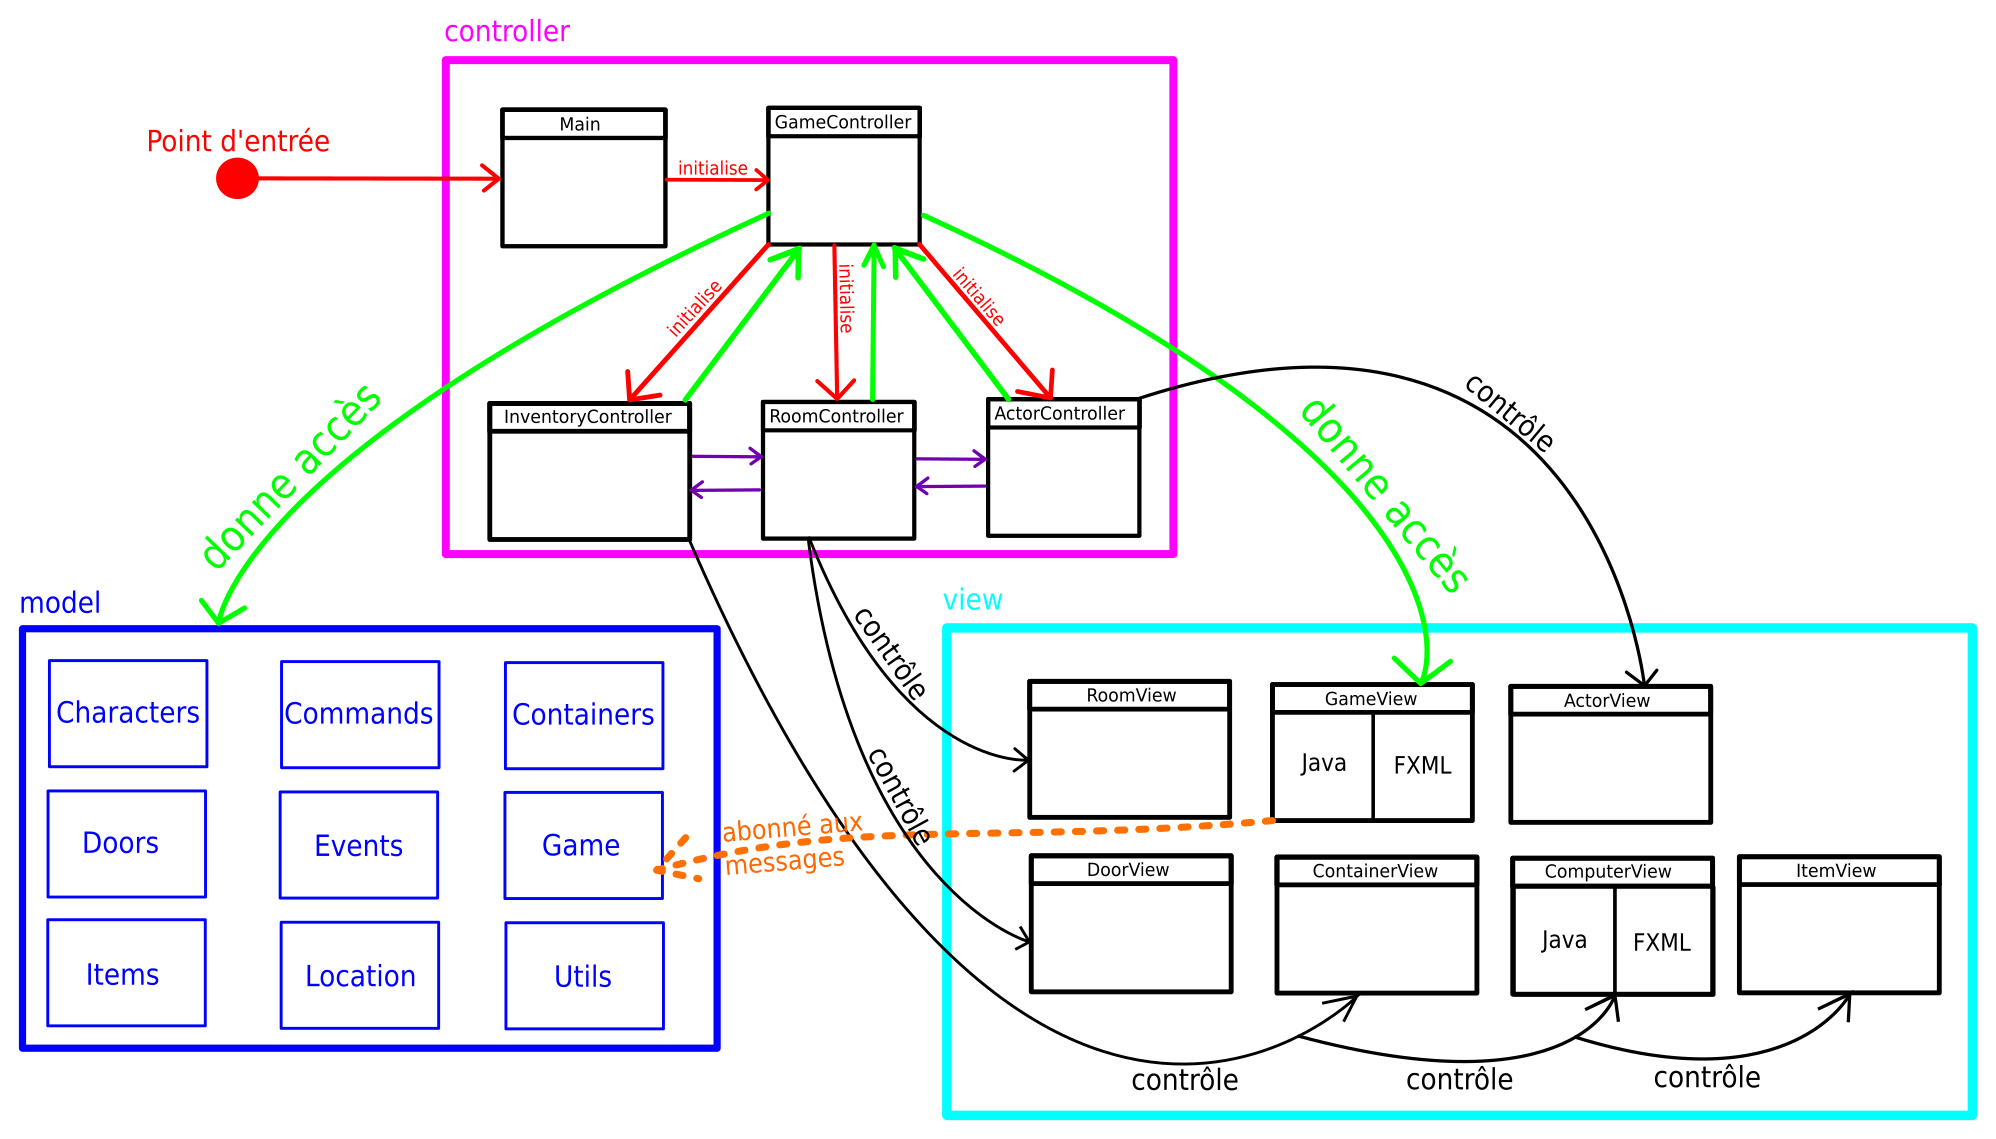
\includegraphics[scale=0.31]{images/structuration.png}
\end{center}

Le jeu se lance avec le \textit{Main} du package \textit{controller}. Ce \textit{Main} initialise le contrôleur général du jeu, appelé \textit{GameController}. Ce contrôleur lui-même lance trois autres contrôleurs spécialisés: le \textit{ActorController}, le \textit{InventoryController} et le \textit{RoomController}.\\

Le but du \textit{GameController} est d'initialiser les gestionnaires d'événements globaux du jeu (manuel d'aide et fin de la partie) et d'offrir une porte d'accès au modèle et à la vue du jeu pour les trois autres contrôleurs plus spécialisés.\\

Aussi, les trois autres contrôleurs ont tous la main sur la vue du jeu (\textit{GameView}) et sur d'autres éléments visuels dont ils sont spécialistes (comme la vue des pièces et des portes - respectivement \textit{RoomView} et \textit{DoorView} - pour le \textit{RoomController})\\

Enfin, ces trois contrôleurs peuvent avoir besoin de communiquer entre eux (flèches violettes sur le schéma). Ceci est le cas, par exemple, pour les fonctions \textit{drop()} et \textit{take()} de l'\textit{InventoryController} qui doit nécessairement connaître la pièce dans laquelle il doit ajouter ou retirer un élément visuel.\\

Quand ils communiquent ils le font toujours en passant par le \textit{GameController} afin d'avoir les données les plus à jour du modèle et de la vue.\\

L'objectif de cette structuration était de recréer de mini modèles MVC au sein d'un modèle MVC plus général. Cette structuration devait permettre d'éviter un contrôleur de jeu trop imposant et d'améliorer la lisibilité du code.\\

Pour terminer, nous noterons l'abonnement de la vue du jeu (\textit{GameView}) aux messages du jeu par le biais d'une interface présente dans le package \textit{Game} du modèle qui envoie les chaînes de caractère du jeu au \textit{MessageListener} enregistré. Ceci nous permettait de continuer de tester le modèle dans la commande (pour y trouver d'éventuels bugs) tout en ne changeant rien au fonctionnement général du jeu.
\newpage


% Section:
\section{Notre démarche dans la construction de cette application}
\medskip

Nous avons commencé le développement dès le lancement du projet le 20 Mars. Ayant un modèle que nous avions beaucoup testé le semestre précédent et qui ne comportait pas de bugs (à notre connaissance), nous avons débuté sur le développement de la vue générale du jeu. Nous avons choisi FXML car nous pensions que c'était l'outil le plus simple pour gérer la création d'une vue aussi complexe.\\

Nous avons ensuite longuement hésité sur la marche à suivre. Nous pensions que le contrôleur associé au document FXML était un "véritable" contrôleur. Aussi nous avions commencé à diviser la vue en 6 FXML différents (un pour la carte du jeu, un autre pour le panneau des acteurs, etc.)\\

En fin de compte il nous a paru plus simple de concevoir le contrôleur associé au FXML comme un moyen d'accéder dans Java aux éléments de la vue FXML. Il s'agissait donc moins d'un contrôleur et bien plus de la "partie Java" de la vue. Nous avons adopté ce point de vue suite à un entretien avec M. Bergey et nous espérons ne pas l'avoir mal interprété.\\


\paragraph{Répartition du travail\\}
Suite à ce travail de conception en collectif nous nous sommes répartis le travail entre nous:
\begin{itemize}
	\item Florian devait réaliser le chargement automatique des pièces (afin d'éviter de coder en dur les vues des 30 pièces du jeu final). Il devait également réaliser la fonction de zoom sur les pièces, les translations avec les sliders et le \textit{binding} du label (cf. élément \textbf{(2)} de l'UI présentée ci-dessus).
	\item Alexis Louail et Vincent Tourenne devaient s'occuper des interactions du joueur avec les aliens et lui-même et ils devaient également s'occuper de l'implantation en GUI de la fonction de sauvegarde et de chargement du jeu.
	\item L'implantation de l'UI de l'inventaire devait être réalisé collectivement à la fin de l'implantation des points évoqués. Cette implantation comprenait les fonctions de prise d'un objet sur le sol, d'affichage de la description des objets et de \textit{give()}, \textit{use()}, \textit{drop()}.\\
\end{itemize}

Cependant, certaines difficultés dont nous faisons la liste ci-après, nous ont amené à revoir cette répartition:
\begin{itemize}
	\item Florian a implanté ses fonctionnalités et celles de l'inventaire
	\item Alexis Louail et Vincent Tourenne ont implanté leur part\\
\end{itemize}
 
\paragraph{Obstacles et difficultés du développement\\}

Durant le développement de ce projet nous avons dû faire face à de nombreuses difficultés:
\begin{itemize}
	\item Les examens de fin d'année
	\item Les autres projets
	\item Un début de stage en 35h dès le 12 Avril pour Florian Legendre
	\item Des difficultés personnelles, des déplacements réguliers et des difficultés matérielles pour Alexis Louail
	\item Des difficultés liées au partage du code sur l'IDE Intellij et aux différentes versions de Java/JavaFx avec Git (fichiers de configuration .idea/)
	\item Nos incompréhensions et fausses routes\\
\end{itemize}

\paragraph{Outils utilisés pour le développent et la gestion de ce projet\\}
L'objectif dans le choix de ces outils était de nous permettre de travailler le plus efficacement possible. Aussi nous avons choisi:
\begin{enumerate}
	\item De versionner notre code sur Git
	\item De nous le partager via un dépôt privé GitHub
	\item De communiquer régulièrement et en temps réel par des salons vocaux ou par messages sur Discord
	\item De nous répartir les bugs détectés via la fonctionnalité des tickets de GitHub
\end{enumerate}


% Section:
\section{Résolution des problèmes de conception}


\newpage

% Section:
\section{Analyse des possibilités d’extension de l’application}



\newpage

% Section:
\section{Erreurs détectées et commentaires}


\newpage

\end{document}